\documentclass[tikz,border=4pt]{standalone}
% Estilo común de los diagramas de bloques (se usa con \input en cada standalone)
\usepackage[defaultsans,scale=0.92]{lato}
\usepackage{libertinust1math}
\usepackage{xcolor,amsmath}
\usepackage{tikz}
\usetikzlibrary{positioning,arrows.meta,calc,shapes.geometric}
\usepackage{../../notacion}
\definecolor{ctrlazul}{HTML}{1E5AA8}\definecolor{ctrlnoche}{HTML}{14213D}
\definecolor{ctrlcoral}{HTML}{D1495B}\definecolor{ctrlverde}{HTML}{2A9D8F}
\definecolor{ctrlambar}{HTML}{E09F3E}\definecolor{ctrlgris}{HTML}{5C677D}
\definecolor{ctrlvioleta}{HTML}{6C4AB6}\definecolor{ctrlteal}{HTML}{0F7173}
\tikzset{
  >={Stealth[length=2.4mm]}, every node/.style={font=\small},
  bloque/.style={draw=ctrlnoche,fill=ctrlazul!7,thick,rounded corners=1.5pt,minimum height=9mm,minimum width=13mm,inner sep=4pt},
  suma/.style={draw=ctrlnoche,thick,circle,inner sep=0pt,minimum size=6mm},
  senal/.style={->,thick,draw=ctrlnoche},
  rot/.style={font=\footnotesize,text=ctrlgris},
}

\begin{document}
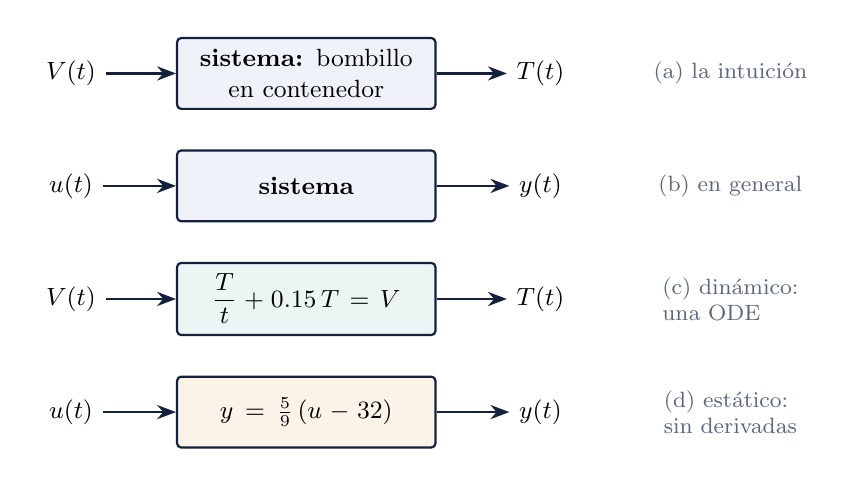
\begin{tikzpicture}[node distance=10mm]
  \matrix[row sep=5mm, column sep=9mm]{
   \node (a1) {$V(t)$}; & \node[bloque,text width=30mm,align=center] (b1) {\textbf{sistema:} bombillo\\ en contenedor}; & \node (c1) {$T(t)$}; & \node[rot] {(a) la intuición};\\
   \node (a2) {$u(t)$}; & \node[bloque,text width=30mm,align=center] (b2) {\textbf{sistema}}; & \node (c2) {$y(t)$}; & \node[rot] {(b) en general};\\
   \node (a3) {$V(t)$}; & \node[bloque,fill=ctrlverde!10,text width=30mm,align=center] (b3) {$\dfrac{\dif T}{\dif t}+0.15\,T=V$}; & \node (c3) {$T(t)$}; & \node[rot,align=left] {(c) dinámico:\\ una ODE};\\
   \node (a4) {$u(t)$}; & \node[bloque,fill=ctrlambar!12,text width=30mm,align=center] (b4) {$y=\frac59\,(u-32)$}; & \node (c4) {$y(t)$}; & \node[rot,align=left] {(d) estático:\\ sin derivadas};\\
  };
  \foreach \i in {1,...,4}{\draw[senal] (a\i)--(b\i); \draw[senal] (b\i)--(c\i);}
\end{tikzpicture}
\end{document}
